%%%%%%%%%%%%%%%%%%%%%%%%%%%%%%%%%%%%%%%%%%%%%%%%%%%%%%
%\section{Human Activity Recognition}
%%%%%%%%%%%%%%%%%%%%%%%%%%%%%%%%%%%%%%%%%%%%%%%%%%%%%%

In this section we describe the implementation of the human acitivity
recognition ('HAR') component on the mobile device.  The algorithmic
foundation of this data mining task have been described in detail in
deliverable D2.2 in section 3.2 ``Mobile Sensing and activity
recognition''. We include a brief summary here (\ref{sec:har_method})
for the sake of completeness. In subsection \ref{sec:har_eval} we
evaluate our method to the on two data sets and compare it to the
state of the art approaches.

\subsection{HAR Method Summary}\label{sec:har_method}


The process of activity recognition uses a pipeline of signal
processing and machine learning techniques. It consists of two phases:
the ``training phase'' and the ``integration phase''. 

\begin{figure}[htbp]
\centering
\subfigure[HAR Training Phase]{
\label{fig:har_overview}
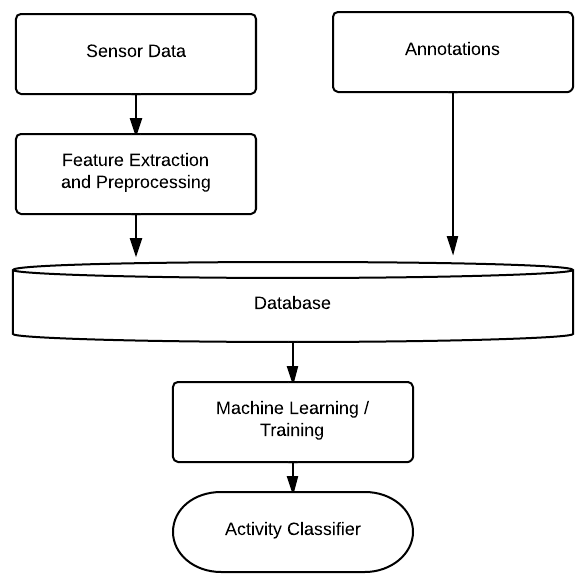
\includegraphics[width=0.5 \textwidth]{img/har/classification_overview.png}
}
\subfigure[HAR Integration Phase]{
\label{fig:integrated_har_overview}
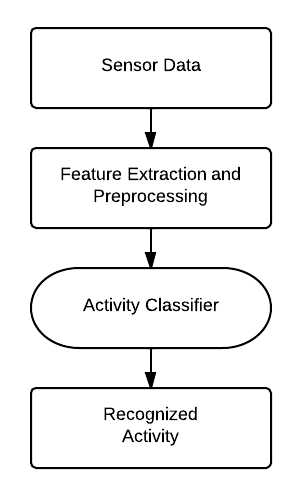
\includegraphics[width=0.25 \textwidth]{img/har/integration_overview.png}
}
\caption{Overview Human Activity Recognition}
\end{figure}


In the training phase (cf. Figure \ref{fig:har_overview}) a group of
volunteers is asked to perform the targeted activities for a certain
amount of time, while recording sensor samples with the device in
their pocket.  The gained training data stored in a database and used
to train a classifier of the activities.

In the integration phase (cf. \ref{fig:integrated_har_overview}), the
trained classifier is embedded into the mobile device.

Both phases rely on the preprocessing steps of "windowing'' and
``feature generation''. The stream of incoming sensor data is divided into
time windows of fixed size (typically 1-10 sec.) and for each window
a set of features is computed. This features are filtering out
relevant information from the raw signal. 

Deliverable D2.2 contains detailed lists of all sensors and features,
that are used in the literature as well as the performance of the
trained classifiers.

\subsection{Component Description}

Architecture Description.

\begin{figure}[htbp]
\centering
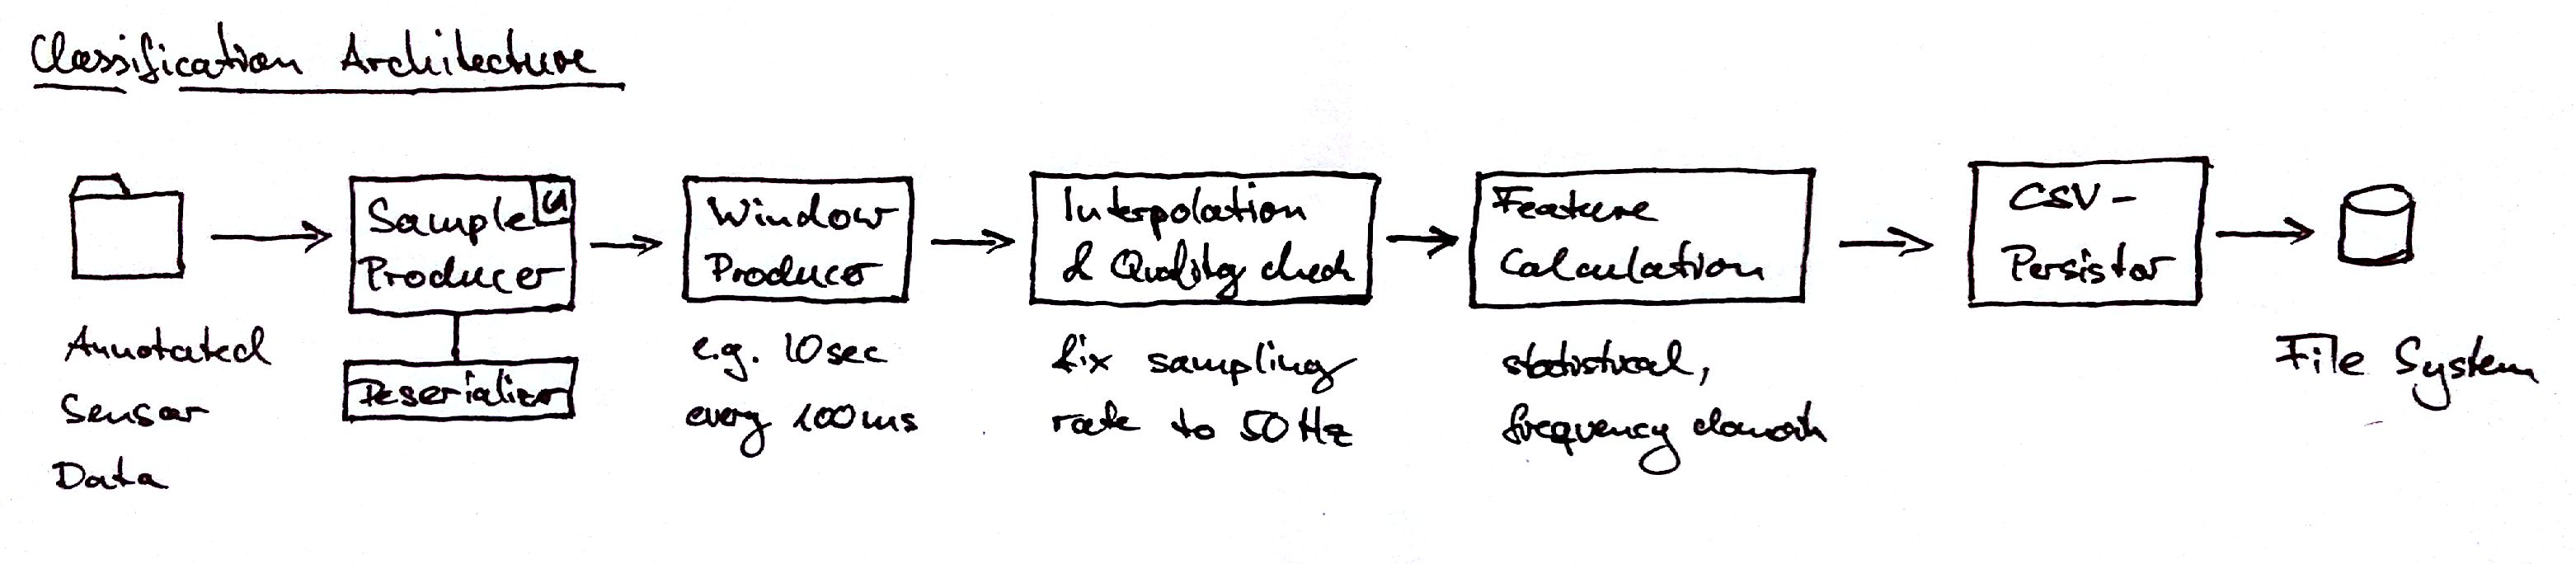
\includegraphics[width=\textwidth]{img/har/classification_architecture.jpg}
\caption{Classification Architecture}\label{fig:classification_architecture}
\end{figure}

\begin{figure}[htbp]
\centering
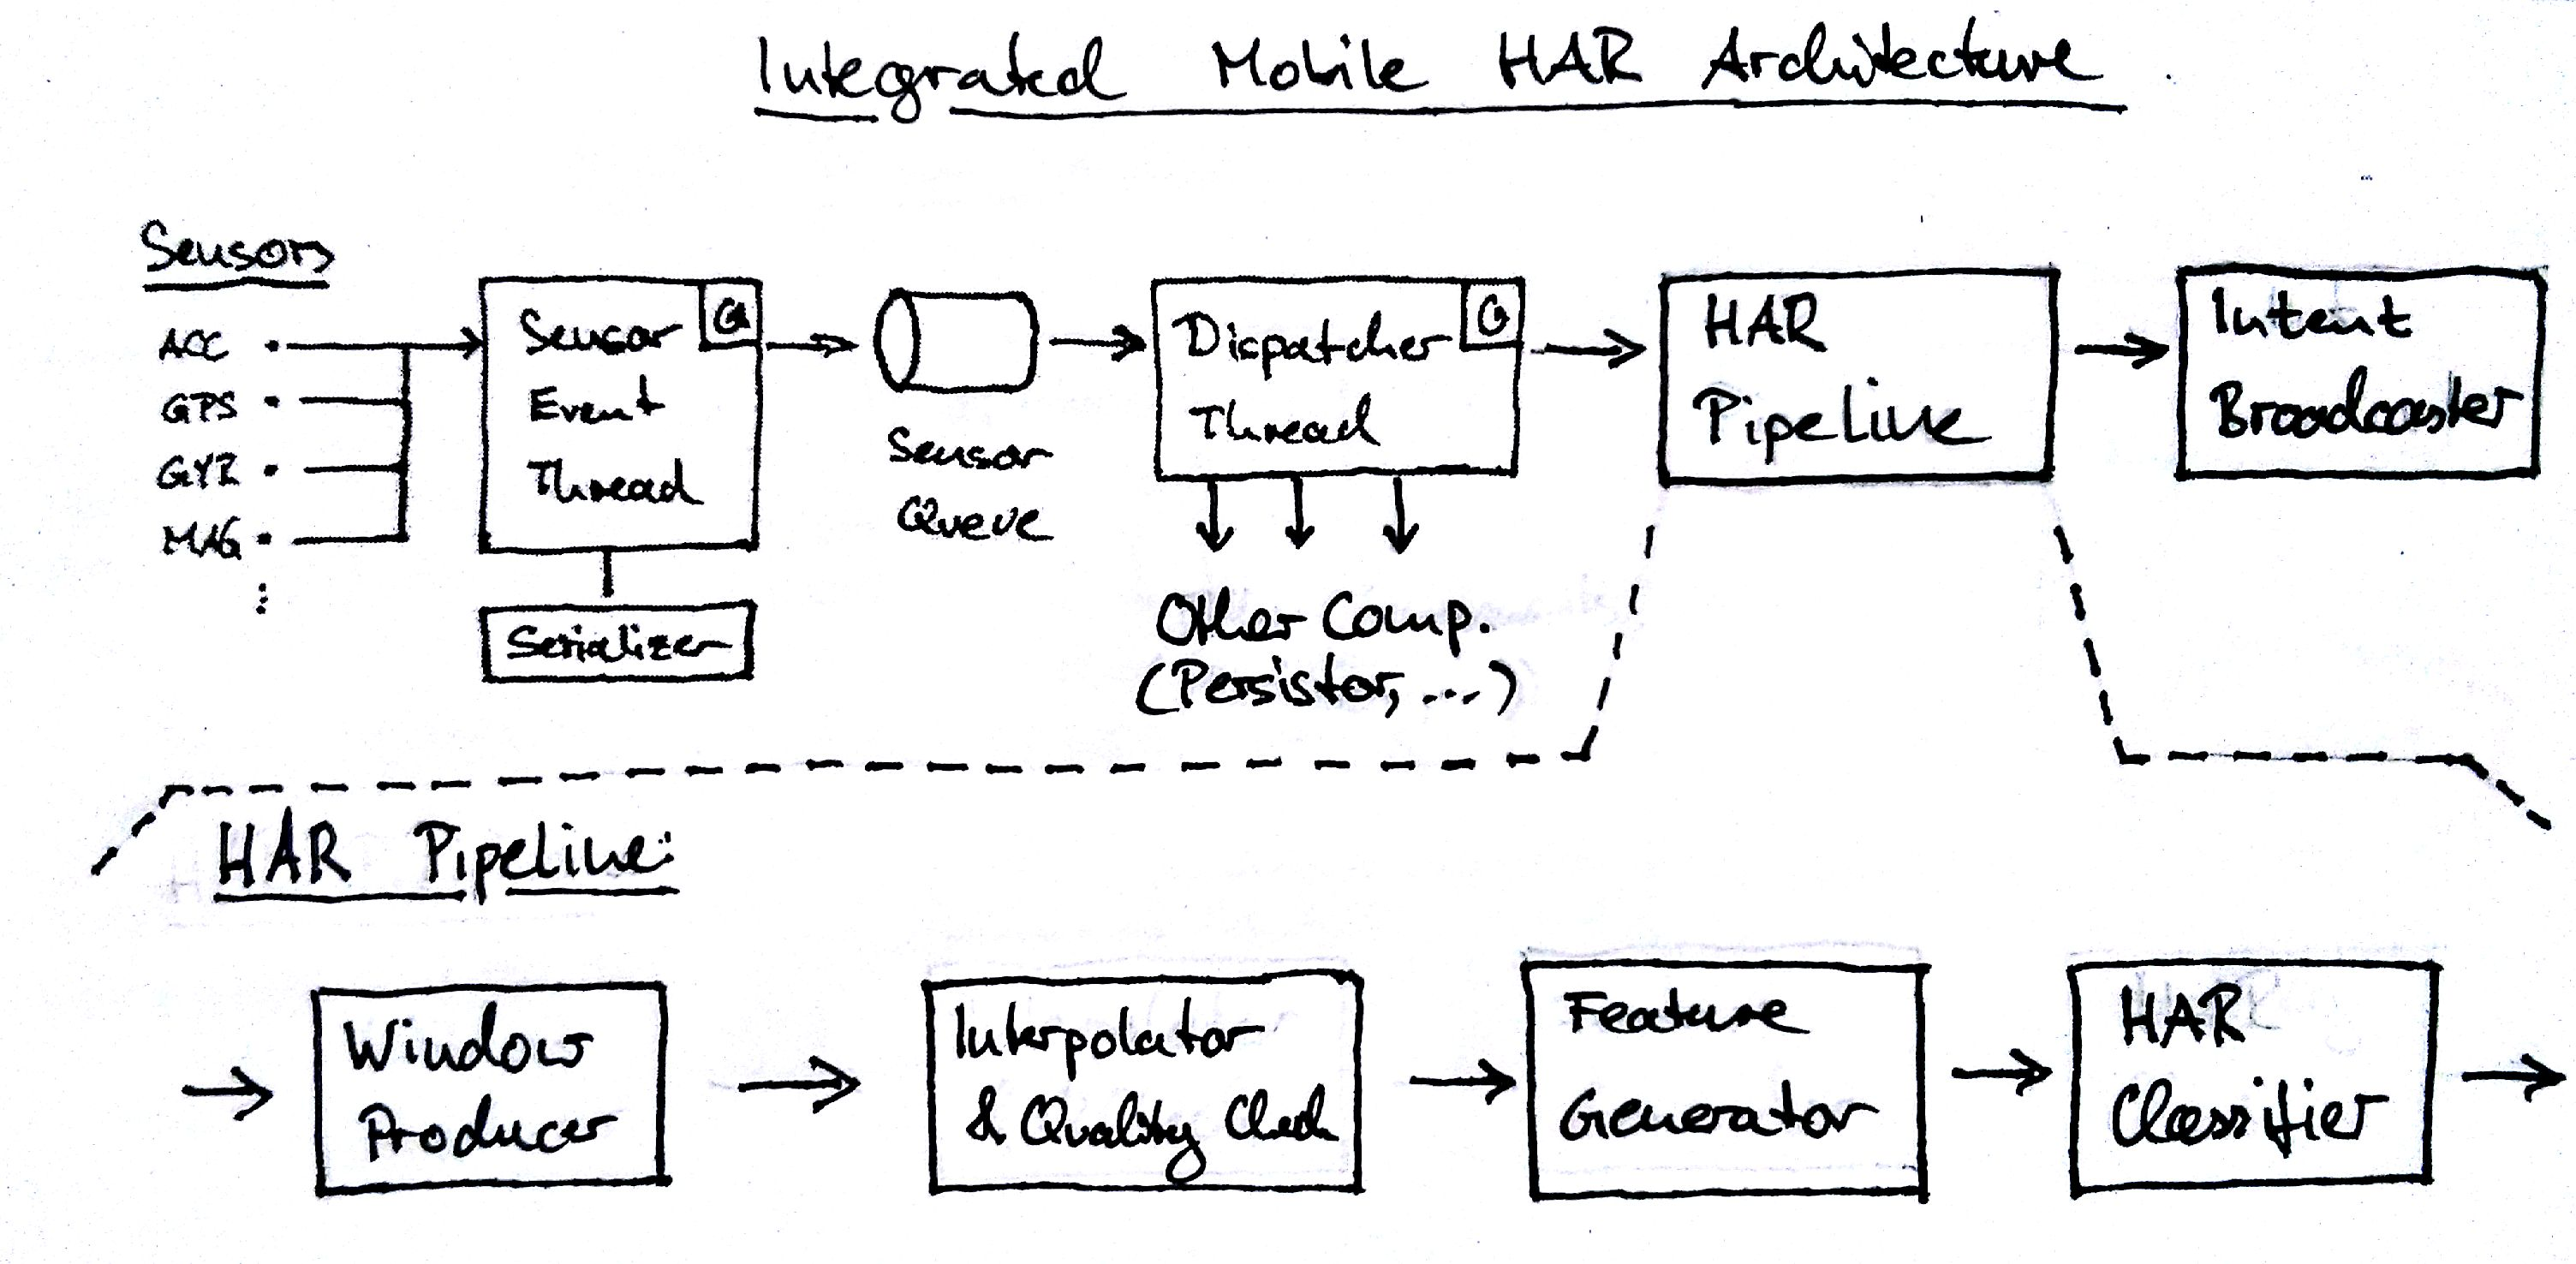
\includegraphics[width=\textwidth]{img/har/integration.jpg}
\caption{Integrated HAR Architecture}\label{fig:integrated_har}
\end{figure}

% TODO CE
% Describe the component implementation.
% This can be done in a similar fashion like the sensor collector
% further up: Add Bullet point list for the individual components.
% And describe them in one or two sentences.
% * Add a list for the features we use in the current implementation
% * Describe how we train the decision tree classifier using WEKA.
%   Add a screenshot of the results. 
% * Describe how we integrate the classifier into the application

% TODO:
% * Describe Dection Tree Classifier [HH]
% * Describe SVM [CERTH]

\subsection{Evaluation}\label{sec:har_eval}

We have evaluated our classifier on two different datasets.  One was
gathered in Koblenz at a data collection event held in December 2013.
The other dataset was obtained from the {\it UCI Machine Learning
  Repository}\footnote{\url{http://archive.ics.uci.edu/ml/datasets/Human+Activity+Recognition+Using+Smartphones}}
and was gathered by Davide Anguita, et. al. \cite{Anguita} in 2012.

Basic Statistics:
\begin{figure}
\centering
\begin{tabular}{|l|c|c|} \hline
Activity  & UCI Dataset & UKOB Dataset \\ \hline
sitting   & 113728      & 80951        \\
standing  & 121984      & 320737       \\
walking   & 110208      & 292024       \\
running   & 0           & 31916        \\
cycling   & 0           & 436106       \\
stairs    & 188800      & 30086        \\
lying     & 124416      & 0            \\ \hline
\end{tabular}
\caption{Number of samples by activity and dataset.}
\end{figure}


\begin{figure}[htbp]
\centering
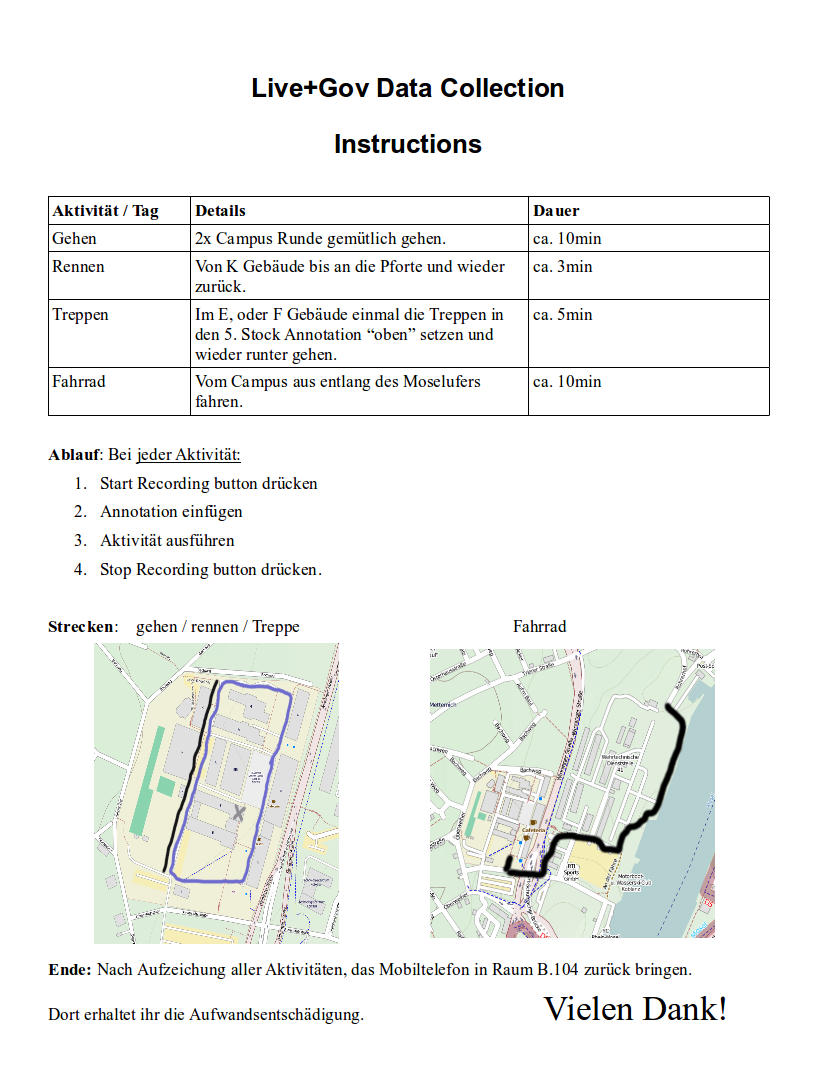
\includegraphics[width=\textwidth]{img/har/data_collection_handout.png}
\caption{Instructions for data collection in German language}\label{fig:data_collection_handout}
\end{figure}





Comparison of our classifier with literature on the basis of external
data sets.



% Describe:
% * Dataset from UKOB
% * Dataset from UCI
%
% * Feature Sets




%%% Local Variables:
%%% mode: latex
%%% TeX-master: "../D1-2"
%%% End:
